\documentclass[10pt,compress,usetitleprogressbar,mathserif]{beamer}
\usepackage[spanish, es-tabla,es-noquoting,es-noshorthands]{babel}
\usepackage{etex}
\usepackage{tikz} % Tikz (para el tema)
\usepackage{showexpl} % ???
\usepackage{amsthm}  %%
\usepackage{amsmath} % Matemáticas
\usepackage{amssymb} %%
\usepackage{graphicx} % Imágenes
\usepackage{adjustbox} % Tamaño de tablas
\graphicspath{{img/}} % Ruta de las imágenes
\usepackage{pgfplotstable} %Tablas
\usepackage{booktabs}% http://ctan.org/pkg/booktabs

\pgfplotstableset{ % Estilo de todas las tablas
sci zerofill,
column type/.add={|}{},
every last column/.style={column type/.add={}{|}},
every head row/.style={before row=\hline},
after row=\hline,
% tex.stackexchange.com/questions/110233
row predicate/.code={%
\pgfmathparse{int(mod(#1,5))}
\ifnum\pgfmathresult=0\relax
\else\pgfplotstableuserowfalse\fi}
}

\usepackage{listings} % Códigos

\definecolor{backg}{HTML}{F2F2F2}    % Fondo
\definecolor{comments}{HTML}{BDBDBD} % Comentarios
\definecolor{keywords}{HTML}{08388c} % Palabras clave
\definecolor{strings}{HTML}{0489B1}  % Strings

\lstset{
language=C++,
basicstyle=\ttfamily\small,
breaklines=true,
backgroundcolor=\color{backg},
keywordstyle=\color{keywords},
commentstyle=\color{comments},
stringstyle=\color{strings},
tabsize=2,
% Acentos, ñ, ¿, ¡ (tex.stackexchange.com/questions/24528)
extendedchars=true,
literate={á}{{\'a}}1 {é}{{\'e}}1 {í}{{\'i}}1 {ó}{{\'o}}1
         {ú}{{\'u}}1 {ñ}{{\~n}}1 {¡}{{\textexclamdown}}1
         {¿}{{?`}}1 {->}{{$\rightarrow$}}1 {=>}{{$\Rightarrow$}}1
}

% Solarized palette
\definecolor{solarizedBase03}{HTML}{002B36}
\definecolor{solarizedBase02}{HTML}{073642}
\definecolor{solarizedBase01}{HTML}{586e75}
\definecolor{solarizedBase00}{HTML}{657b83}
\definecolor{solarizedBase0}{HTML}{839496}
\definecolor{solarizedBase1}{HTML}{93a1a1}
\definecolor{solarizedBase2}{HTML}{EEE8D5}
\definecolor{solarizedBase3}{HTML}{FDF6E3}
\definecolor{solarizedYellow}{HTML}{B58900}
\definecolor{solarizedOrange}{HTML}{CB4B16}
\definecolor{solarizedRed}{HTML}{DC322F}
\definecolor{solarizedMagenta}{HTML}{D33682}
\definecolor{solarizedViolet}{HTML}{6C71C4}
\definecolor{solarizedBlue}{HTML}{268BD2}
\definecolor{solarizedCyan}{HTML}{2AA198}
\definecolor{solarizedGreen}{HTML}{859900}

\usetheme{epstfg}
\setbeamertemplate{note page}[compress]
\setbeamertemplate{itemize subitem}{\tiny\raise1.5pt\hbox{\donotcoloroutermaths$\blacktriangleright$}}
\title{Práctica 3}
\author{Pablo Baeyens \and Antonio Checa \and Iñaki Madinabeitia \and José Manuel Muñoz \and Darío Sierra}
\date{Algorítmica}
\def\inline{\lstinline[basicstyle=\ttfamily]}

\begin{document}
\maketitle

\begin{frame}{Índice}
  \tableofcontents
\end{frame}
\section{Contenedores en un barco}

\begin{frame}{Problema}
Rellenar un buque con carga limitada ($K$) con un conjunto
de contenedores $c_1,\dots, c_n$ con pesos $p_1, \dots, p_n$.

\begin{description}
 \item[Entrada:] Vector de pesos de los contenedores, $p$ y capacidad total $K$
 \item[Salida:] Vector con los contenedores elegidos
\end{description}
\end{frame}

\begin{frame}[fragile]{Estructura de datos}
\lstinputlisting[firstline=11, lastline=19]{cpps/contenedores.cpp}
\end{frame}

\subsection{Maximizar el número de contenedores cargados}

\begin{frame}{Solución}
\begin{itemize}
  \item Basta coger los contenedores de menor peso hasta rellenar el buque
  \item Emparejamos cada elemento con su posición y ordenamos en función de los pesos.
  \item Una vez ordenados, rellenamos hasta agotar la capacidad.
  \item \textbf{Eficiencia:} $O(n\log(n))$
\end{itemize}
\end{frame}

\begin{frame}[fragile]{Código}
\lstinputlisting[firstline=39, lastline=52]{cpps/contenedores.cpp}
\note{\texttt{menor} compara dos contenedores según su peso, indicando cuál es menor}
\end{frame}

\begin{frame}{Optimalidad}
Este criterio siempre halla la solución con un mayor número de contenedores.

Vamos a razonar por reducción al absurdo.

\pause
Partimos de nuestra solución  $o_1, \dots, o_k$ del algoritmo anterior. Estos contenedores son los menores entre todos los posibles.

Suponemos otra solución, $s_1, \dots, s_m$, una solución del problema, con mayor número de contenedores. Es decir, $m > k$.


\begin{center}
	%% Luego borráis esto pero por dios que el que exponga no se le olvide explicar el final de la demostración que viene en la memoria
	\textit{Explicasión en pisarra}
\end{center}
%%TODO: ¿Lo ponemos? ¿Cómo?
%% Antonio: Creo que lo mejor es dejar las hipótesis y el planteamiento, y que el que exponga lo explique en la pizarra con detalle
%% Lo he puesto como he visto, pero no me convence mucho porque hay mucho texto junto, si queréis cambiarlo
\end{frame}

\subsection{Maximizar el número de toneladas cargadas}

\begin{frame}{Estrategia}
\begin{itemize}
  \item Cogemos el contenedor de mayor peso que quepa en el buque.
  \item El algoritmo es muy similar al del apartado anterior.
\end{itemize}
\end{frame}

\begin{frame}[fragile]{Código}
\lstinputlisting[firstline=54, lastline=66]{cpps/contenedores.cpp}
\end{frame}

\begin{frame}{Perspectiva}
	Hemos querido comparar el algoritmo Greedy anterior (que coge en cada momento el contenedor que más aumenta el peso total) con uno que encuentra la mejor solución siempre.
	\vspace{1cm}
	
	De esta forma, podremos ver las ventajas que presenta enfocar las soluciones de una forma simple.
\end{frame}

\begin{frame}{Otro algoritmo}
	A continuación colocamos el algoritmo que encuentra siempre el óptimo:
	
	\begin{itemize}
		\item Está basado en la fuerza bruta
		\item Recorre todas las posibilidades y se queda con la mejor.
		\item \textbf{Eficiencia:} $O(n!)$
	\end{itemize}	
\end{frame}

\begin{frame}[fragile]{Código}
	\lstinputlisting[firstline=84, lastline=107]{cpps/contenedores.cpp}
	%% TODO: No cabe, así que o lo ponemos de otra manera, o lo acortamos o no lo ponemos :/
\end{frame}

\begin{frame}{Comparativa}
	Es fácil ver que el algoritmo greedy es más eficiente que el óptimo, pero el óptimo tiene asegurada la mejor respuesta.
	
	Para poder compararlos mejor, hemos hecho las gráficas de comapración.
\end{frame}

\begin{frame}{Comparativa}
	%% Inaki: Primera gráfica en función de Capacidad / Tiempo de ejecución
\end{frame}

\begin{frame}{Comparativa}
	%% Inaki: Segunda gráfica en función de Capacidad / Peso total
\end{frame}

\begin{frame}{Conclusión}
	Este es un ejemplo en el que es posible que nos interese trabajar con algoritmos greedy si quisiéramos conseguir una solución rápida a un problema grande.
\end{frame}

%% TODO: Justificación chusquera de por qué hemos elegido esta heurística

%% TODO: Explicar el algoritmo de fuerza bruta

\section{El problema del viajante de comercio}

\begin{frame}{Problema}
Hallar el recorrido con distancia mínima en un conjunto de
ciudades que pase por todas las ciudades y regrese al punto inicial.

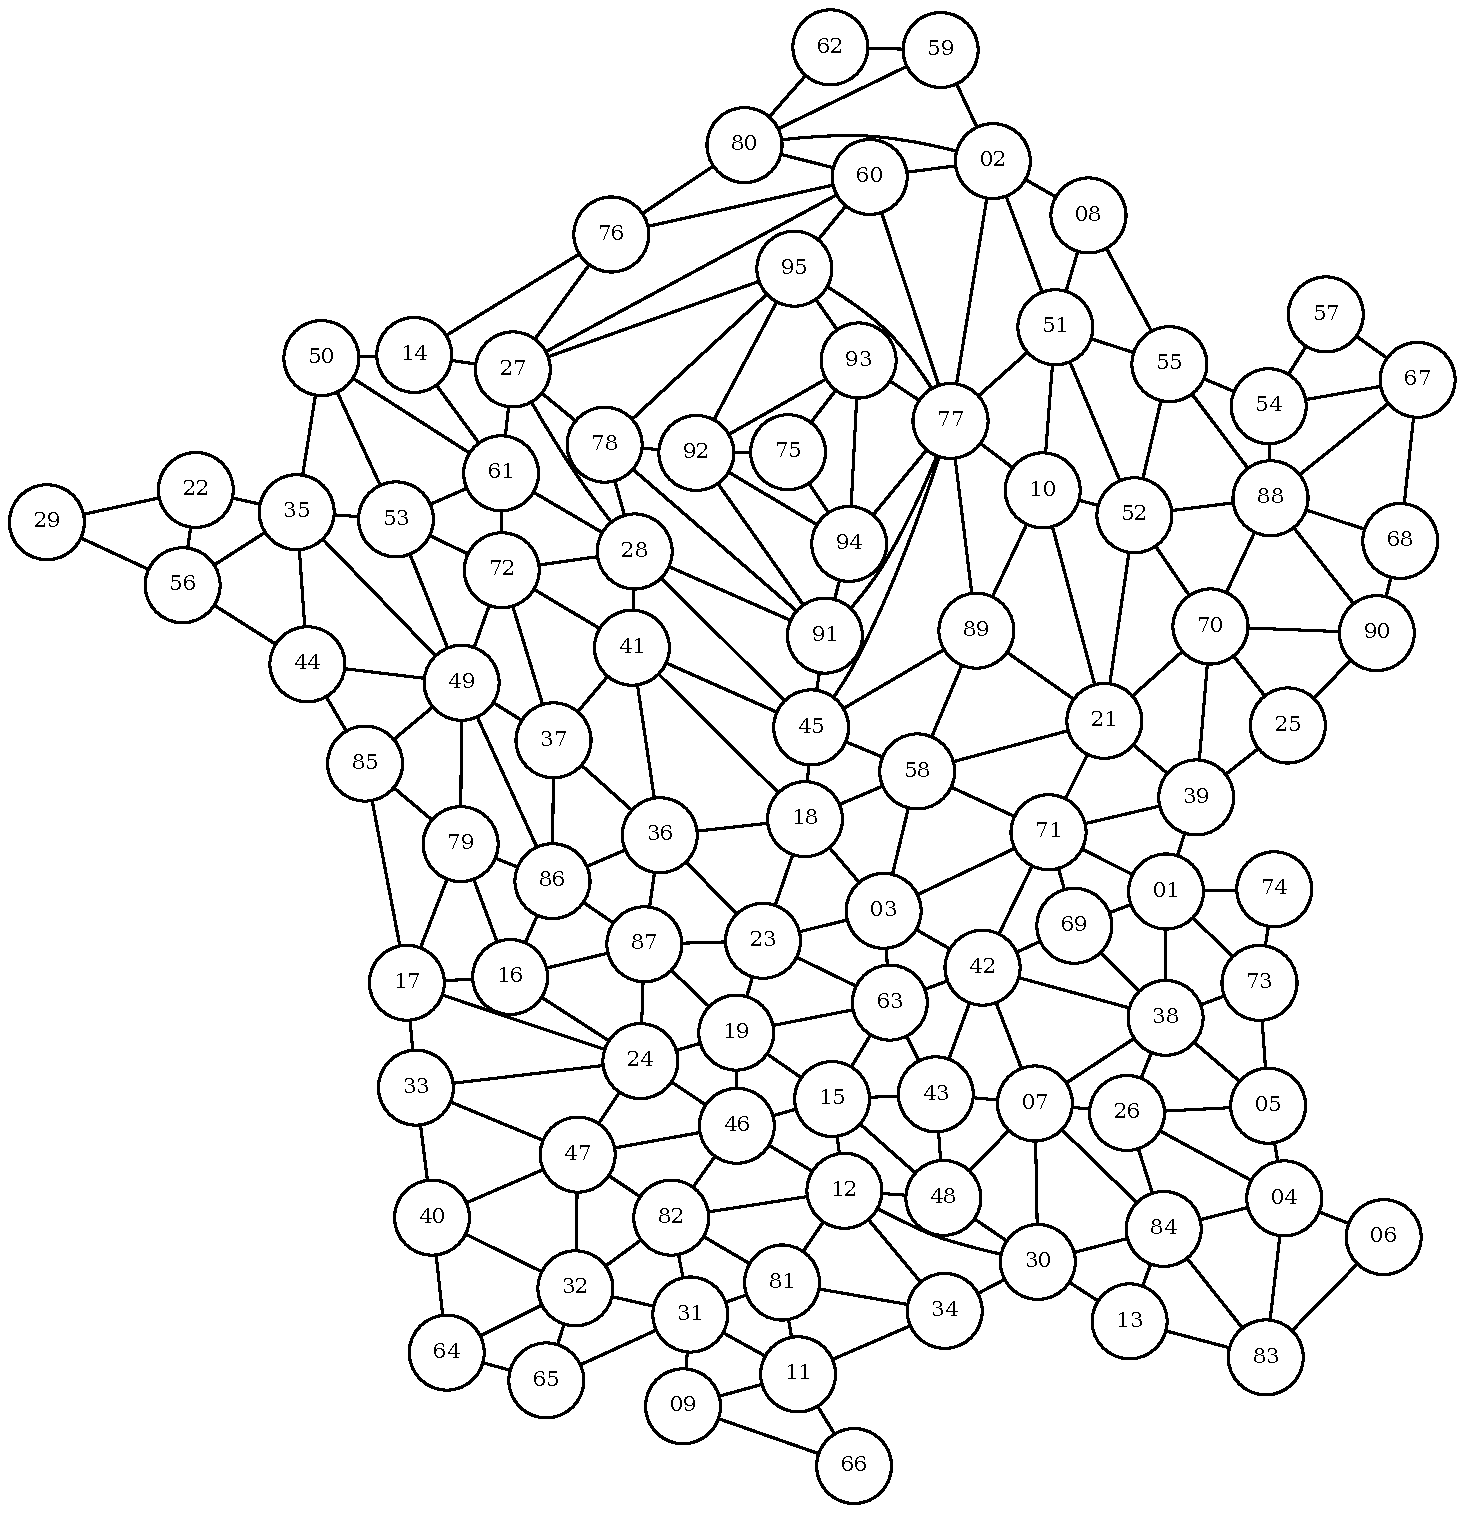
\includegraphics[width=.5\textwidth]{img/Francia} \centering
\end{frame}

\begin{frame}{Algoritmos}
\begin{description}
 \item[Entrada:] Ficheros con ciudades indicadas como puntos en el plano según sus
 coordenadas.
 \item[Salida:] \texttt{vector<int>} con el orden en el que se recorren las ciudades.
\end{description}
\end{frame}

% TODO: todo lo posterior

\begin{frame}{\texttt{Grafo}}
Un grafo consta de:

\begin{itemize}
  \item Una \textbf{cantidad de nodos}: \texttt{nodos}.
  \item Una \textbf{matriz de pesos}: \texttt{lados}.
\end{itemize}
\end{frame}

\subsection{Ramificación y acotación}

\begin{frame}{Algoritmo general}
  Iniciamos:
  \begin{itemize}
    \item La cola con la solución parcial \texttt{[0]}
    \item La mejor solución con un algoritmo \textit{greedy} (vecino más cercano)
  \end{itemize}
\end{frame}

\begin{frame}{Algoritmo general}
  Mientras la cola no esté vacía, coge el primer elemento:
  \begin{itemize}
    \item Si \textbf{puede formarse una solución completa}, comprueba si es mejor que la mejor encontrada. En tal caso actualizala y borra los nodos con peor cota.
    \item En \textbf{otro caso}, para cada ciudad no visitada forma una nueva solución parcial. Añádela a la cola si su cota es mejor que la mejor solución.
  \end{itemize}
\end{frame}

\subsubsection{Cotas}

\begin{frame}{Cota del mínimo}
  Calcular la longitud del recorrido inicial y suma la menor distancia de cada ciudad no incluida en la solución parcial con sus relacionadas.
\end{frame}

\begin{frame}{Arbol generador}
  Calcular la longitud del recorrido que se lleva hasta ese momento, y suma la longitud del árbol generador minimal de los nodos que faltan junto al último nodo del camino. Además, se suma la mínima longitud del primer nodo a otro más.

  %% Aquí pintad en pizarra que si no, no lo entiende ni dios, y es una tontería
\end{frame}

\subsection{Vuelta atrás}

\begin{frame}{Backtracking}
  Desde un nodo inicial, vamos tomando todas las posibilidades mediante una llamada recursiva. Si al añadir un nodo hace que el camino mida más que nuestra mejor longitud hasta el momento, se deja esa posibilidad, y se vuelve atrás.
\end{frame}

\begin{frame}[fragile]{Llamada inicial backtracking}
\begin{lstlisting}
vector<int> tsp_backtracking(const Grafo<peso_t>& g) {
	vector<int> primera_solucion = tsp_greedy(g);
	int mejor_longitud = longitud(primera_solucion,g);
	vector<int> inicial = {0};
	vector<int> solucion; // Se modifica

	tsp_back_rec(solucion,inicial,mejor_longitud,g);

	return solucion;
}
\end{lstlisting}
\end{frame}

\subsection{Comparativa de los algoritmos}

\begin{frame}{5 ciudades (tiempos)}
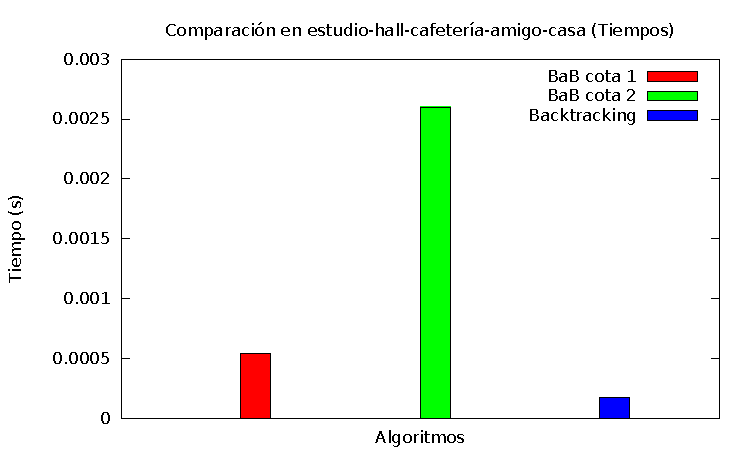
\includegraphics[width=\textwidth]{img/barras_e-h-c-a-c5_t}
\end{frame}

\begin{frame}{5 ciudades (nodos expandidos)}
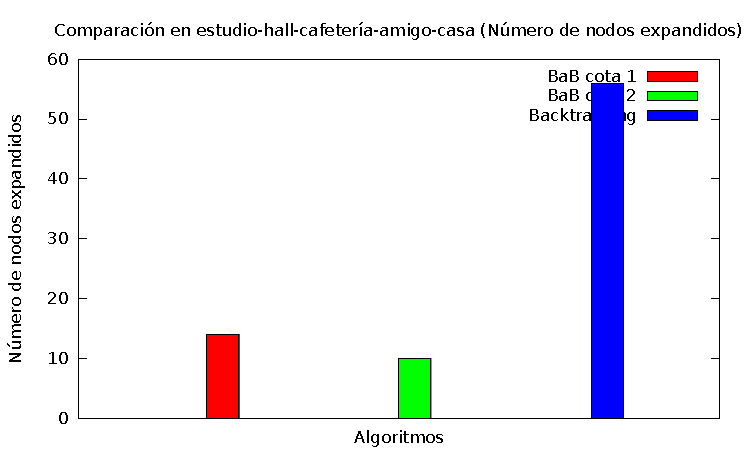
\includegraphics[width=\textwidth]{img/barras_e-h-c-a-c5_nodos}
\end{frame}

\begin{frame}{5 ciudades (Podas)}
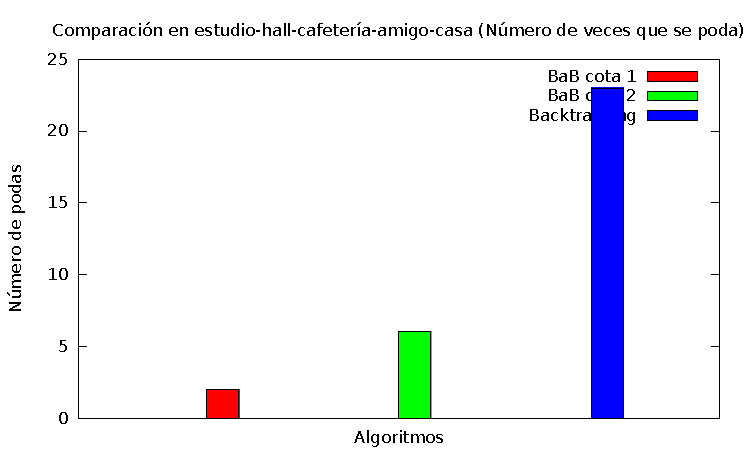
\includegraphics[width=\textwidth]{img/barras_e-h-c-a-c5_poda}
\end{frame}

\begin{frame}{5 ciudades (Cola)}
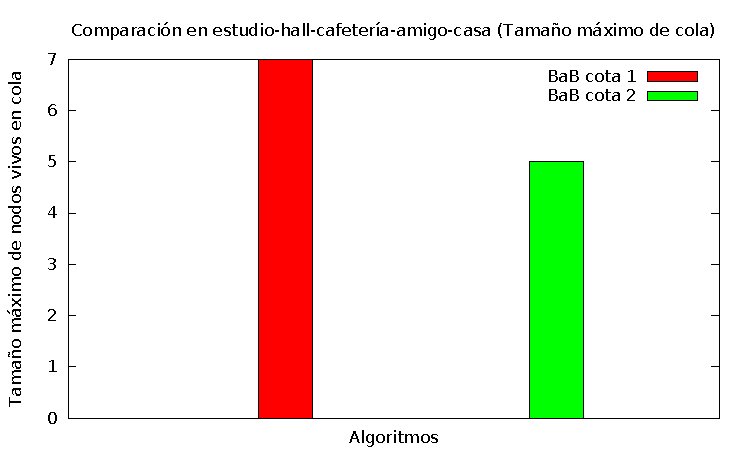
\includegraphics[width=\textwidth]{img/barras_e-h-c-a-c5_cola}
\end{frame}

\begin{frame}{10 ciudades (tiempos)}
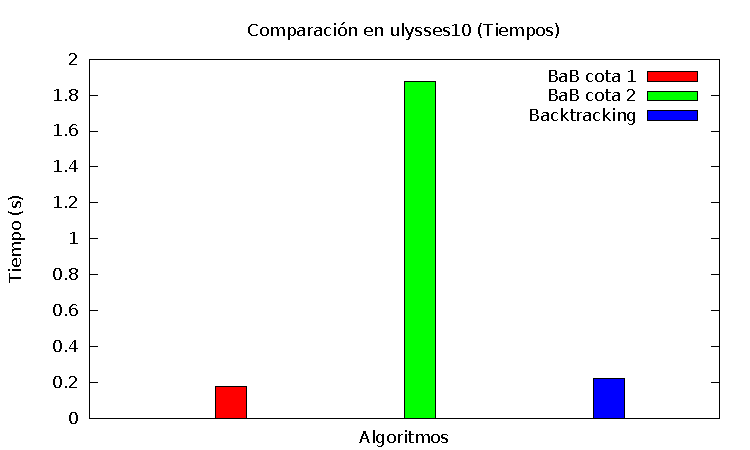
\includegraphics[width=\textwidth]{img/barras_ulysses10_t}
\end{frame}

\begin{frame}{10 ciudades (nodos expandidos)}
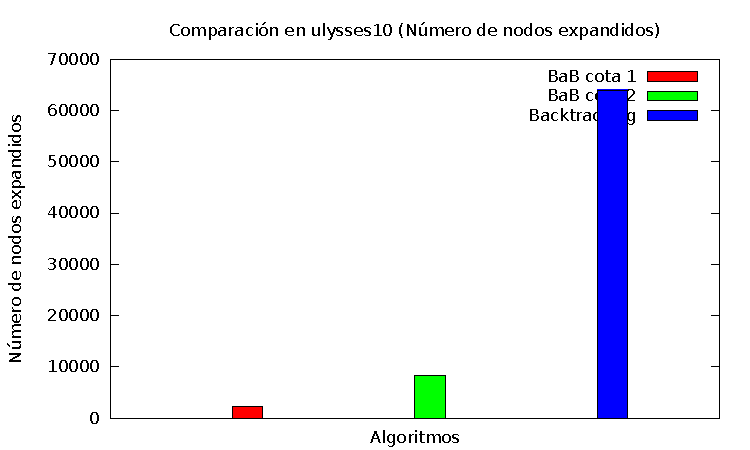
\includegraphics[width=\textwidth]{img/barras_ulysses10_nodos}
\end{frame}

\begin{frame}{10 ciudades (Podas)}
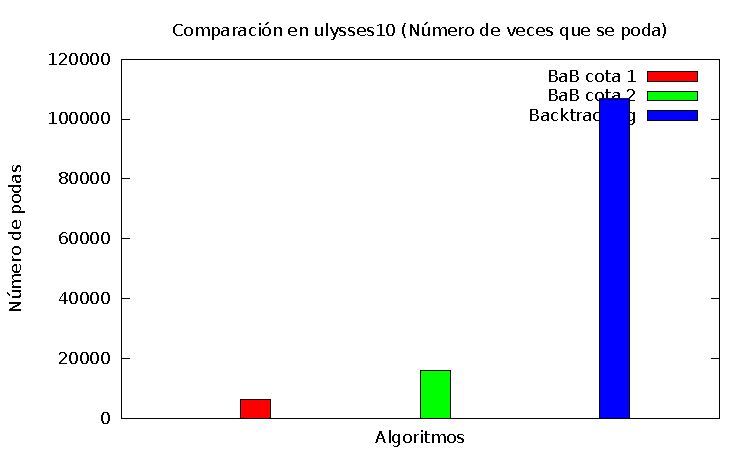
\includegraphics[width=\textwidth]{img/barras_ulysses10_poda}
\end{frame}

\begin{frame}{10 ciudades (Cola)}
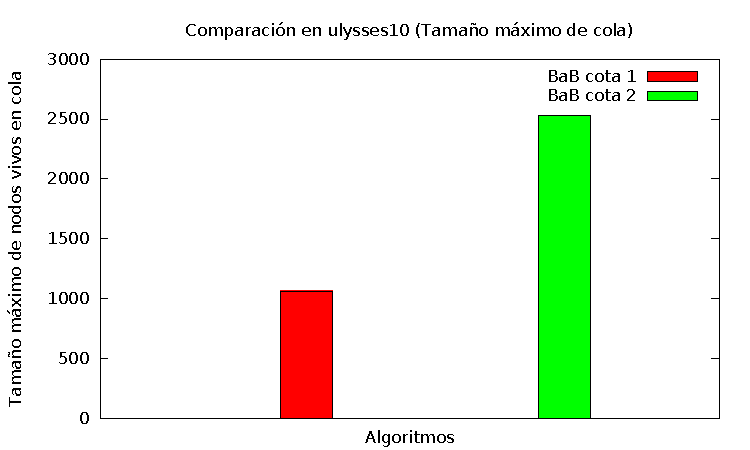
\includegraphics[width=\textwidth]{img/barras_ulysses10_cola}
\end{frame}

\begin{frame}{12 ciudades (tiempos)}
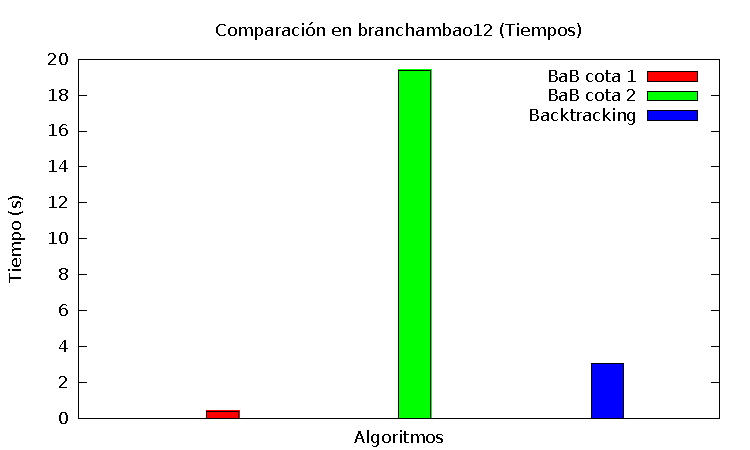
\includegraphics[width=\textwidth]{img/barras_branchambao12_t}
\end{frame}

\begin{frame}{12 ciudades (nodos expandidos)}
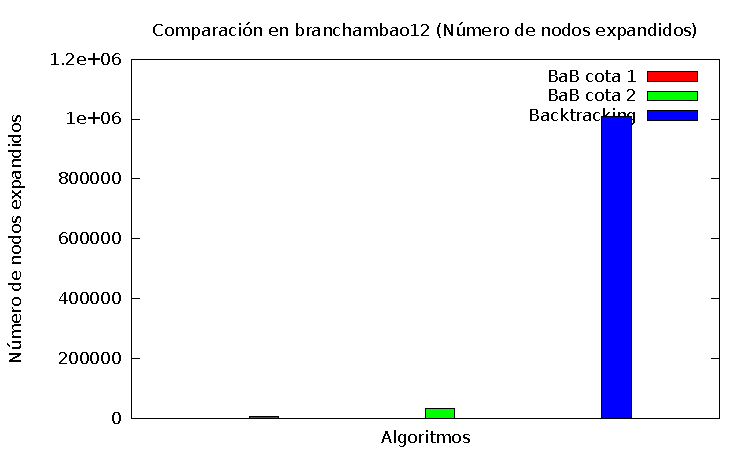
\includegraphics[width=\textwidth]{img/barras_branchambao12_nodos}
\end{frame}

\begin{frame}{12 ciudades (Podas)}
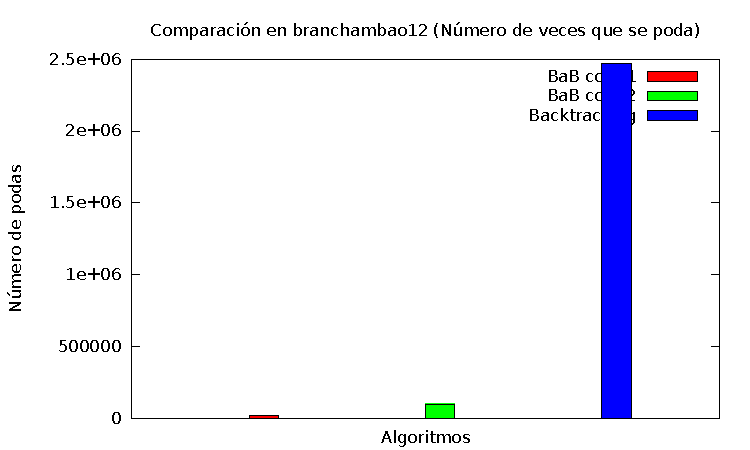
\includegraphics[width=\textwidth]{img/barras_branchambao12_poda}
\end{frame}

\begin{frame}{12 ciudades (Cola)}
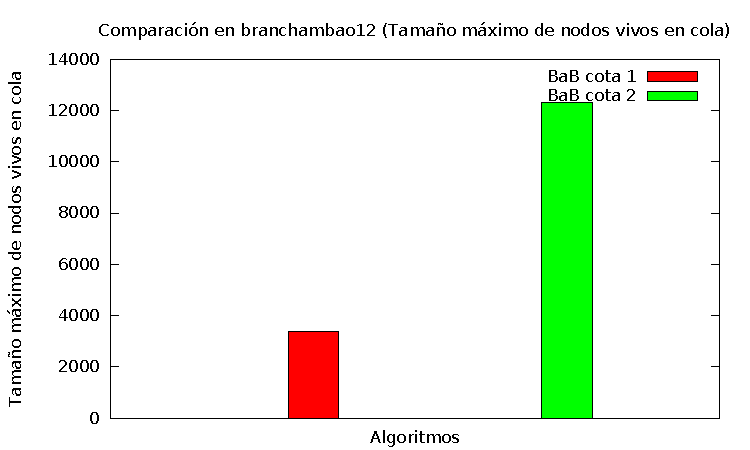
\includegraphics[width=\textwidth]{img/barras_branchambao12_cola}
\end{frame}

\end{document}
